\documentclass[a4paper]{article}
\usepackage[utf8]{inputenc}
\usepackage{tikz}
\usetikzlibrary{quantikz}
\usepackage{physics}
\usepackage[english]{babel}
\usepackage{pgfplots}
\usepgfplotslibrary{units}
\usetikzlibrary{patterns}
\usepackage{siunitx}
\usetikzlibrary{angles, quotes}
\usepackage{amssymb}
\usetikzlibrary{angles, arrows.meta, quotes}
\pgfplotsset{compat=1.17}
\usepackage{amsthm}
\usepackage{amsmath}
\usepackage{graphicx}

\newtheorem{theorem}{Theorem}
\usepackage{minted}
\usepackage[most]{tcolorbox}
\definecolor{lightgreen}{rgb}{0.56, 0.93, 0.56}
\definecolor{moonstoneblue}{rgb}{0.45, 0.66, 0.76}

\graphicspath{ {./} }

\newtcblisting{myminted}{%
    listing engine=minted,
    minted language=c,
    listing only,
    breakable,
    enhanced,
    minted options = {
        linenos,
        breaklines=true,
        breakbefore=.,
        fontsize=\footnotesize,
        numbersep=2mm
    },
    overlay={%
        \begin{tcbclipinterior}
            \fill[gray!25] (frame.south west) rectangle ([xshift=4mm]frame.north west);
        \end{tcbclipinterior}
    }
}

\begin{document}
	\title{

	\vspace{1cm}
	\Huge Quantum Teleportation Algorithm
	}

	\vspace{1cm}

	% if you are the only author, you might use the following
	% \author{Name of student}

	% Insert here your name and correct mail address
	\author{\Large {Rutvij Menavlikar} \Large \\  \ \ 2019111032
	\date{November 23, 2020}
	\vspace{0.5cm}}

	\maketitle
	\setlength{\parindent}{0pt}

\vspace{8cm}
\begin{abstract}
\begin{center}
\normalsize
This document is an introduction to the Quantum teleportation protocol and some of the concepts associated with it.
\end{center}
\end{abstract}
	\newpage
	\tableofcontents
	\newpage

\maketitle

\section{The need for a separate Teleportation Protocol}
\indent Given two Quantum Computers, where one of these computers has a qubit in some qubit state, and now it wants to transfer this qubit state to the other computer. \\ \\
For a classical computer, this procedure is pretty straightforward. You measure the bit, which can be in exactly two states, i.e. \textbf{0} and \textbf{1}, and send this data over to the other computer via some network. And after receiving this data, the other computer can construct it's bit identical to the bit of the first computer. \\ \\
But the problem in quantum computers is that a qubit can exist in infinite states($\mathbb{C}^{2}$), but measuring that qubit destroys it's state and reduces it to exactly one of 2 orthogonal qubit states. \\
Let the qubit to be teleported be $q_0$, and let
$$\ket{q_{0}} = \alpha \ket{0} + \beta \ket{1} \text{ where } \alpha,\beta \in \mathbb{C}$$
Now measuring the qubit $q_0$, and storing the result in the classicla bit $c_0$,
\begin{center}
\begin{quantikz}
\lstick{$\ket{q_0}$} & \meter{0/1} \arrow[r] & \rstick{$c_0$}
\end{quantikz}
\end{center}
The bit $c_0$ exists in only two state, i.e. \textbf{0}(with probability $|\alpha|^2$) and \textbf{1}(with probability $|\beta|^2$). \\
The initial qubit $q_0$ has been destroyed and since infinite number of states have been stored as one of two states, data is lost and it is impossible to rebuild the same qubit in the other quantum computer. \\
Also, note that creating the qubit repeatedly and measuring it to get $|\alpha|^2$ and $|\beta|^2$ is not enough either. Because for a complex number $z$, even when we know $|z|$, there are infinite possibilities for the value of $z$. \\ \\
Hence, measuring and sending over the results of measurement will not work every time. \\

\section{No Cloning Theorem}
Another need for a Quantum Teleportation Protocol is the No Cloning Theorem. \\
In classical computers we can easily copy the state of 1 bit to another bit without measuring the bit and creating the state in another bit. But, this is not the case in a quantum computer. This operation is prevented by the No Cloning theorem. \\ \\
\begin{theorem} [No Cloning Theorem]
It is impossible to create an independent and identical copy of an arbitrary unknown quantum state.
\end{theorem}
\begin{proof}
First, we define inner product of two quantum states $\ket{\psi}$ and $\ket{\phi}$ as $\bra{\psi}\ket{\phi}$, where
$$\ket{\psi}=\alpha_{0}\ket{0}+\alpha_{1}\ket{1}\text{, }\ket{\phi}=\beta_{0}\ket{0}+\beta_{1}\ket{1}\text{ and }\alpha_{0},\alpha_{1},\beta_{0},\beta_{1}\in\mathbb{C}$$
then,
$$\bra{\psi}\ket{\phi}=\overline{\alpha_{0}}\beta_{0}+\overline{\alpha_{1}}\beta_{1}$$
where for a complex number $z$, $\overline{z}$ is it's complex conjugate.\\
We also observe that,
\begin{equation*}
\begin{split}
\bra{\psi\psi}\ket{\phi\phi} & = \bra{\ket{\psi}\otimes\ket{\psi}}\ket{\ket{\phi}\otimes\ket{\phi}} \\
& = \bra{(\alpha_{0}^{2}\ket{00}+\alpha_{0}\alpha_{1}\ket{01}+\alpha_{0}\alpha_{1}\ket{10}+\alpha_{1}^{2}\ket{11})}\ket{(\beta_{0}^{2}\ket{00}+\beta_{0}\beta_{1}\ket{01}+\beta_{0}\beta_{1}\ket{10}+\beta_{1}^{2}\ket{11})}\\
& = \overline{\alpha_{0}^{2}}\beta_{0}^{2}+\overline{\alpha_{0}\alpha_{1}}\beta_{0}\beta_{1}+\overline{\alpha_{0}\alpha_{1}}\beta_{0}\beta_{1}++\overline{\alpha_{1}^{2}}\beta_{1}^{2}\\
& = (\overline{\alpha_{0}}\beta_{0}+\overline{\alpha_{1}}\beta_{1})^{2}\\
& = \bra{\psi}\ket{\phi}^{2}
\end{split}
\end{equation*}
Let us assume that $\ket{\psi}$ and $\ket{\phi}$ are not orthogonal, i.e. $\bra{\phi}\ket{\psi}\neq0$\\
If possible, there exists a unitary transformation $U$, such that for any quantum state $\ket{\phi}$, $U\ket{\phi}\otimes\ket{0}=\ket{\phi}\otimes\ket{\phi}$\\
Now, we have
$$U\ket{\psi}\otimes\ket{0}=\ket{\psi}\otimes\ket{\psi}\text{ and }U\ket{\phi}\otimes\ket{0}=\ket{\phi}\otimes\ket{\phi}$$
Now we consider
\begin{align*}
\bra{\psi}\ket{\phi} & = \bra{\ket{\psi}\otimes\ket{0}}\ket{\ket{\phi}\otimes\ket{0}} \\
& = (\ket{\psi}\otimes\ket{0})(\ket{\phi}\otimes\ket{0}) \\
& = (\ket{\psi}\otimes\ket{0})U`\text{ . }U(\ket{\phi}\otimes\ket{0}) && \text{(U is a unitary transformation,} \\ &&& \text{and hence it is reversible)} \\
& = (\ket{\psi}\otimes\ket{\psi})(\ket{\phi}\otimes\ket{\phi}) \\
& = \bra{\psi}\ket{\phi}^{2}
\end{align*}
And since $\ket{\psi}$ and $\ket{\phi}$ are not orthogonal, $\bra{\psi}\ket{\phi}=1$. \\
And this is not the case for every pair of quantum states $\ket{\psi}$ and $\ket{\phi}$. \\
\textbf{Contradiction} \\ \\
Hence, it is impossible to create an independent and identical copy of an arbitrary unknown quantum state.
\end{proof}

\section{Pre-requisites to Quantum Teleportation}
Suppose the sender quantum computer has a qubit $\ket{S}$ in an unknown quantum state, and we want to transfer this quantum state to the receiver quantum computer's qubit $\ket{R}$. \\
We would need to set $\ket{R}$ to $\ket{0}$ and the sender computer would require a qubit $\ket{I}$, when $\ket{I}$ and $\ket{R}$ are in a bell state, i.e. $\ket{IR}=\frac{1}{\sqrt{2}}\ket{00}+\frac{1}{\sqrt{2}}\ket{11}$. \\
\begin{center}
\begin{quantikz}
\lstick{$\ket{S}$} & \qw & \qw & \qw \\
\lstick{$\ket{I}$} & \gate{H} & \ctrl{1} & \qw \\
\lstick{$\ket{R}$} & \qw & \targ{} & \qw \\
\end{quantikz} \\
\end{center}
We will also require two classical bits $crx$ and $crz$ which will be sent from the sender quantum computer to the receiver quantum computer. \\
Hence, the circuit before applying the teleportation protocol will be \\
\begin{center}
\begin{quantikz}
\lstick{$\ket{S}$} & \qw & \qw & \qw \\
\lstick{$\ket{I}$} & \gate{H} & \ctrl{1} & \qw \\
\lstick{$\ket{R}$} & \qw & \targ{} & \qw \\
\lstick{$crz$} & \cw & \cw & \cw \\
\lstick{$crx$} & \cw & \cw & \cw \\
\end{quantikz} \\
\end{center}

\section{The Quantum Teleportation Protocol}
Now that we have the two classical bits and the three qubits, two of which are in a bell state, we are ready to implement the teleportation protocol. \\
Note that because of the No Cloning theorem, when we teleport a qubit, we destroy it's quantum state in one place and recreate the exact same quantum state on another qubit. \\
We first apply a CNOT gate with control and target qubits as $\ket{S}$ and $\ket{I}$ respectively, and then we apply a Hadamard gate to the qubit $\ket{S}$. \\
\begin{center}
\begin{quantikz}
\lstick{$\ket{S}$} & \qw & \qw & \ctrl{1} & \gate{H} & \qw \\
\lstick{$\ket{I}$} & \gate{H} & \ctrl{1} & \targ{} & \qw & \qw \\
\lstick{$\ket{R}$} & \qw & \targ{} & \qw  & \qw & \qw \\
\lstick{$crz$} & \cw & \cw & \cw & \cw & \cw \\
\lstick{$crx$} & \cw & \cw & \cw & \cw & \cw \\
\end{quantikz} \\
\end{center}
If we assume that $\ket{S}=\alpha\ket{0}+\beta\ket{1}$ where $\alpha,\beta\in\mathbb{C}$, then after these operations we get the combined state of the qubits as
$$\ket{SIR}=\frac{\alpha}{2}\ket{000}+\frac{\beta}{2}\ket{001}+\frac{\beta}{2}\ket{010}+\frac{\alpha}{2}\ket{011}+\frac{\alpha}{2}\ket{100}-\frac{\beta}{2}\ket{101}-\frac{\beta}{2}\ket{110}+\frac{\alpha}{2}\ket{111}$$
We now measure the qubits $\ket{S}$ and $\ket{I}$ and store the result in the classical bits $crz$ and $crx$ respectfully. \\
\begin{center}
\begin{quantikz}
\lstick{$\ket{S}$} & \qw & \qw & \ctrl{1} & \gate{H} & \meter{0/1} \vcw{3} & \qw & \qw \\
\lstick{$\ket{I}$} & \gate{H} & \ctrl{1} & \targ{} & \qw & \qw & \meter{0/1} \vcw{3} & \qw \\
\lstick{$\ket{R}$} & \qw & \targ{} & \qw  & \qw & \qw & \qw & \qw \\
\lstick{$crz$} & \cw & \cw & \cw & \cw & \cw & \cw & \cw \\
\lstick{$crx$} & \cw & \cw & \cw & \cw & \cw & \cw & \cw \\
\end{quantikz} \\
\end{center}
The following table denotes the state of $\ket{R}$ for each value of ($crz$, $crx$). \\
\begin{center}
\begin{tabular}{ |c|c|c| }
\hline
$crz$ & $crx$ & $\ket{R}$ \\
\hline \hline
0 & 0 & $\alpha\ket{0}+\beta\ket{1}$ \\
\hline
0 & 1 & $\beta\ket{0}+\alpha\ket{1}$ \\
\hline
1 & 0 & $\alpha\ket{0}-\beta\ket{1}$ \\
\hline
1 & 1 & $\alpha\ket{1}-\beta\ket{0}$ \\
\hline
\end{tabular}
\end{center}
To rebuild $\ket{R}$ to the original value of $\ket{S}$, we can use the calculated values of $crz$ and $crx$ as conditions to apply the Z gate and X gate on $\ket{R}$. \\
\begin{center}
\begin{quantikz}
\lstick{$\ket{S}$} & \qw & \qw & \ctrl{1} & \gate{H} & \meter{0/1} \vcw{3} & \qw & \qw & \qw & \qw \\
\lstick{$\ket{I}$} & \gate{H} & \ctrl{1} & \targ{} & \qw & \qw & \meter{0/1} \vcw{3} & \qw & \qw & \qw \\
\lstick{$\ket{R}$} & \qw & \targ{} & \qw  & \qw & \qw & \qw & \gate{Z} \vcw{1} & \gate{X} \vcw{2} & \qw \\
\lstick{$crz$} & \cw & \cw & \cw & \cw & \cw & \cw & \cw & \cw & \cw \\
\lstick{$crx$} & \cw & \cw & \cw & \cw & \cw & \cw & \cw & \cw & \cw \\
\end{quantikz} \\
\end{center}

\section{Implementation of Quantum Protocol}
The code for this protocol has been written in qiskit and a script to simulate the teleportation using the QASM simulator have been included in the project files. \\ \\
The entanglement in bell state and then further operations of CNOT and Hadamard gate can all be replaced by one 3 bit quantum gate T on which measurements are done to complete the teleportation protocol. \\
\begin{center}
\begin{quantikz}
\lstick{$\ket{S}$} & \gate[wires=3][3cm]{T} & \meter{0/1} \vcw{3} & \qw & \qw & \qw & \qw \\
\lstick{$\ket{I}$} &  & \qw & \meter{0/1} \vcw{3} & \qw & \qw & \qw \\
\lstick{$\ket{R}$} &  & \qw & \qw & \gate{Z} \vcw{1} & \gate{X} \vcw{2} & \qw \\
\lstick{$crz$} & \cw & \cw & \cw & \cw & \cw & \cw \\
\lstick{$crx$} & \cw & \cw & \cw & \cw & \cw & \cw \\
\end{quantikz} \\
\end{center}
In the case where $qubit 0$ is $\ket{S}$, $qubit 1$ is $\ket{R}$ and $qubit 2$ is $\ket{I}$. \\
When $qubit 0$ is in the state (Bloch Sphere notation) \\ 
\begin{figure}[htp]
\centering
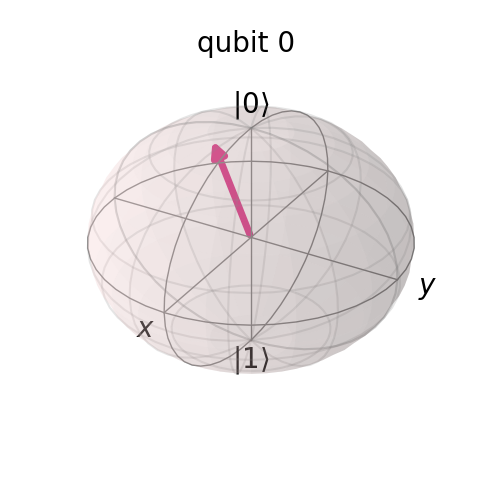
\includegraphics[scale=0.8]{before.png}
\caption{Initial Quantum state of sender quantum computer's qubit}
\label{fig:before}
\end{figure} \\
After completing the teleportation the protocol, the final states of the qubits are (in Bloch Sphere notation) \\
\begin{figure}[htp]
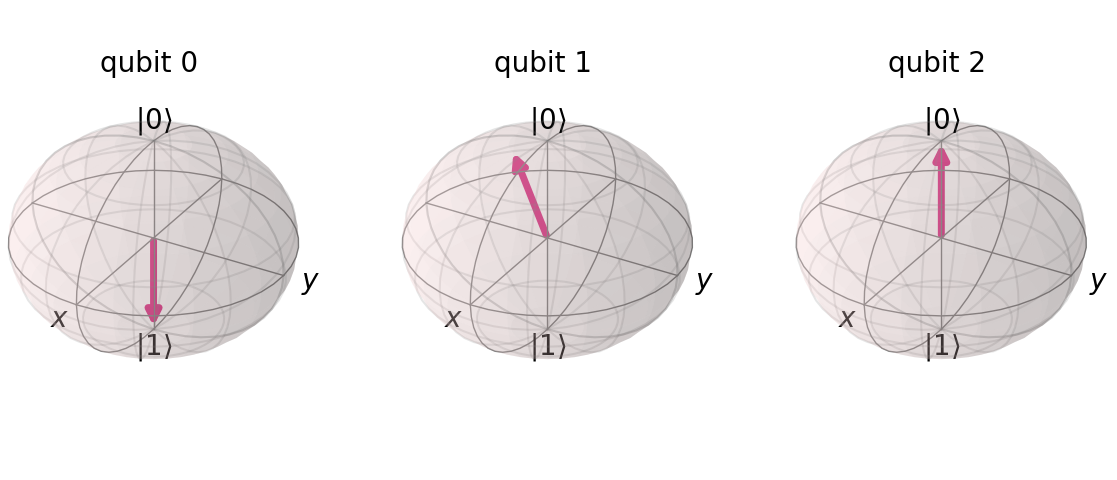
\includegraphics[width=\textwidth]{after.png}
\caption{Final Quantum state of the sender quantum computer's qubit, the intermediate qubit and the receiver quantum computer's qubit}
\label{fig:after}
\end{figure} \\
\\ \\ \\ \\
And as you can observe, VOILA! We have achieved Quantum Teleportation!

\section{An Important Note}
Given the fact that when we measure the qubits $\ket{S}$ and $\ket{I}$, the effects of it are immdiately observed on $\ket{R}$, one may assume that this protocol allows communications to take place faster than the speed of light. \\
But this is not accurate. \\ \\
While the quantum state of $\ket{R}$ may be updated instantaneously, and may also have happened before light would have arrived to it's location, it is impossible to exactly determine which of the four possible quantum states to use without knowing the two classical bits. \\
And these Classical bits arrive at a speed less than or equal to the speed of light. \\
Hence, Quantum Teleportation Algorithm cannot achieve communication faster than the speed of light.

\end{document}